%卒業論文用雛形
\documentclass[a4j,12pt,oneside,openany]{jsbook}
% 英語なら以下を使う.
%\documentclass[a4j,12pt,oneside,openany,english]{jsbook}

\usepackage[dvipdfmx]{graphicx}
\usepackage{amssymb}
\usepackage{amsmath}
\usepackage{latexsym}

%jsbook を report っぽくするスタイルファイル
\usepackage{book2report}
%定理,補題,系,例題,証明などや英語用の定義がされています.
%自分なりにいじってください.
\usepackage{thesis}
% 具体的には以下のように定義されています.
% 英語の定理環境
%  \newtheorem{theorem}{Theorem}[chapter]
%  \newtheorem{lemma}{Lemma}[chapter]
%  \newtheorem{proposition}{Proposition}[chapter]
%  \newtheorem{corollary}{Corollary}[chapter]
%  \newtheorem{definition}{Definition}[chapter]
%  \newtheorem{example}{Example}[chapter]
%  \newtheorem{proof}{Proof}
% 日本語の定理環境
%  \newtheorem{theorem}{定理}[chapter]
%  \newtheorem{lemma}{補題}[chapter]
%  \newtheorem{proposition}{命題}[chapter]
%  \newtheorem{corollary}{系}[chapter]
%  \newtheorem{definition}{定義}[chapter]
%  \newtheorem{example}{例}[chapter]
%  \newtheorem{proof}{証明}
% 証明には番号をつけず,最後は Box で終わります.

% 英語で,見出しのフォントが気に入らなかったら
%\renewcommand{\headfont}{\bfseries}

% ページ数が少ないときはここを大きくしてごまかそう!!効果絶大!!
\renewcommand{\baselinestretch}{1.0}

\begin{document}
\chapter{運転支援システムの説明}
\label{ch:2}

\par
タクシーの営業方法には,待ち営業と流し営業の二種類がある.
待ち営業とは,駅前やホテルの入り口などの乗り場で待機して乗客を獲得する営業方法である.
この方法の利点は,乗り場で待っていればタクシーは乗客をほぼ確実に獲得できるということ,乗客を探すためにタクシーを空車の状態で走らせる必要がないということである.
一方,欠点は,待機所でのタクシーの待ち行列が渋滞の原因の一つになっているということ,待ち営業を行える場所以外での乗客獲得の機会を逃している場合があるということである.
流し営業とは,乗客の獲得が期待できる経路を走行して乗客を獲得する営業方法である.
この方法の利点は,乗務員の経験と勘があれば待ち営業よりも乗客を獲得できる機会が多いということ,乗客からすれば,わざわざタクシー乗り場に向かわずともタクシーを利用できるということである.
一方,欠点は,空車状態での走行時間が長いと燃料費がかかってしまい利益が減ってしまうということ,乗客獲得の確実性がないということである.
現在,タクシー事業者は,各乗務員に対して流しでの営業を行うことを推奨している.
しかしながら,ほぼ確実に乗客を獲得できるという利点から,待ち営業を行う乗務員が多いのが現状である.

\par
最近では,すべてのタクシーにGPSが搭載されており,乗客を乗せた時刻・位置などが日々データベースに蓄積されている.
流し営業の欠点は乗客獲得の確実性がないことだが,乗務員に対してデータベースの情報を活用した有益な情報が提示できる仕組みを構築すれば,流しでの営業を行う乗務員の増加が期待できる.
本章では,タクシー営業の生産性の向上を目的として企業との共同開発で作成したソフトウェアのシステム構成と乗務員に提示する情報について説明を行う.

\section{システム構成}
 \label{sec:2_1}
\par
ソフトウェアはスマートフォン上で実行され,乗務員に提示される.
各乗務員が所有しているスマートフォンを利用することで,タクシー事業者はカーナビを購入する経費を抑えられる利点がある.
一方,スマートフォンの画面は小さいので,乗務員が使いやすいように搭載する機能や提示する情報を選定する必要がある.

\par
図\ref{fig:2_1_1}は実際に作成したソフトウェアの実行画面である.
\begin{figure}[tp]
 \centering
 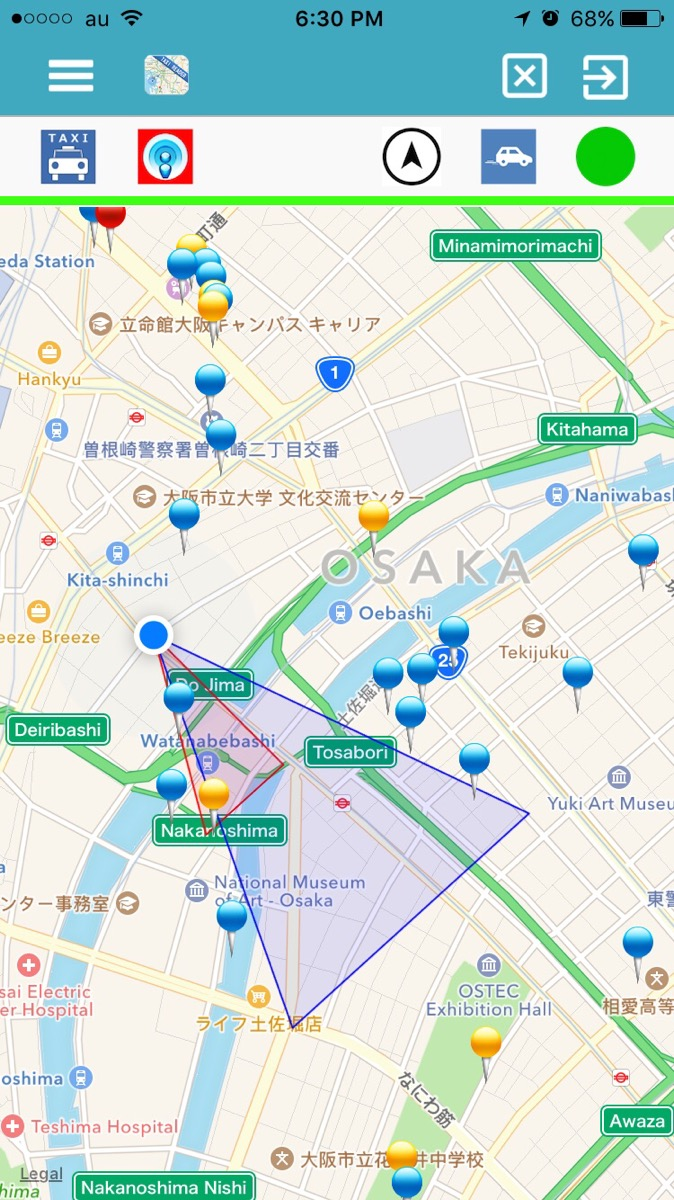
\includegraphics[keepaspectratio, width=60mm]
 {Graphics/chapter2/201603311830.jpg}
 \caption{ソフトウェアの実行画面}
 \label{fig:2_1_1}
\end{figure}
乗務員がこのソフトウェアを利用する手順は以下のとおりである.
まず,ソフトウェアを起動して画面上で提供される情報を参考にして流し営業を行う.
もし,乗客を乗せた場合は画面右上にある緑色のサークルのアイコンをタップする.
その時,乗客を乗せた時刻と位置情報はデータサーバーに送信され,サークルのアイコンは緑色から赤色に変化する.
ソフトウェア上でのタクシーの状態も空車から実車に変化する.
緑色のサークルのアイコンはタクシーが空車状態であることを表し,赤色のサークルのアイコンは実車状態であることを表す.
乗客を下ろした場合は,もう一度サークルのアイコンをタップしてタクシーの状態を実車から空車に戻す.
その時,乗客を降ろした時刻と位置情報はデータサーバーに送信され,サークルのアイコンは赤色から緑色に変化する.

\par
データサーバーには乗降車を行った位置と時刻の情報以外にも,一定時間が経過した場合や,一定距離を走行した場合の位置と時刻の情報も送信される.
表\ref{tab:tab2_1_1}は実際にデータサーバーに保存される乗降車データである.
\begin{table}[t]
  \begin{center}
    \caption{データサーバーに保存される乗降車データ}
    \begin{tabular}{|l|l|l|l|l|l|} \hline
      乗車時刻 & 乗車緯度 & 乗車経度 & 降車時刻 & 降車緯度 & 降車経度 \\ \hline \hline
      2016-11-06 02:18:08 & 34.6612 & 135.5029 & 2016-11-06 02:30:21 & 34.6494 & 135.5194 \\
      2016-11-06 02:40:40 & 34.6678 & 135.5091 & 2016-11-06 02:47:48 & 34.6709 & 135.5390 \\
      2016-11-06 03:03:59 & 34.6693 & 135.5063 & 2016-11-06 03:11:49 & 34.6701 & 135.5062 \\ \hline
    \end{tabular}
    \label{tab:tab2_1_1}
  \end{center}
\end{table}
データ量削減のために空車のときの位置情報や,実車のときの走行経路の情報は保存されない.
このソフトウェアは乗務員の運転支援を行うだけでなく,タクシーの走行履歴を取得しデータサーバーに送信する役割もある.

\section{画面上で提示される情報}
\label{sec:2_2}
\par
ソフトウェア上では,タクシー事業者が定めた時間幅が1単位時間に設定されており,1単位時間ごとにソフトウェアの画面が更新される.
画面上で提供される情報は以下の5つである.

1つ目は,過去に乗車実績のあった箇所を表すピン(図\ref{fig:2_1_1}を参考)である.
2つ目は,ピンに基づいた利己的な走行方向を示す赤色の三角形のオブジェクト(図\ref{fig:2_1_1}を参考)である.
3つ目は,ピンに基づいた推奨される走行方向を示す青色の三角形のオブジェクト(図\ref{fig:2_1_1}を参考)である.
4つ目は,古典的なニューラルネットワークにより予測した需要の中で値が大きい箇所を表す情報である.
5つ目は,営業領域内の電車の遅延や事故のような交通情報である.
以下では,実際に乗務員に表示できるようにした情報について詳しく説明する.
\subsection{ピン情報}
\par
図\ref{fig:2_1_1}の画面内にあるピンは過去に乗車実績のあった箇所を示す.
実装では,現在の日付から2,3,4週間前の日の,現在の時刻から2分前から4分後までの間に乗車実績のあった箇所をピンで表示するようにした.
ピンの色は3種類あり,青,黄,赤の順に乗車時間が10分未満,10分以上20分未満,20分以上であった乗降車記録を示している.
ピンが密集している箇所は乗客を獲得できる頻度が高いと言える.

\begin{figure}[t]
    \begin{tabular}{c}
      %---- 最初の図 ---------------------------
      \begin{minipage}[h]{1\hsize}
        \centering
        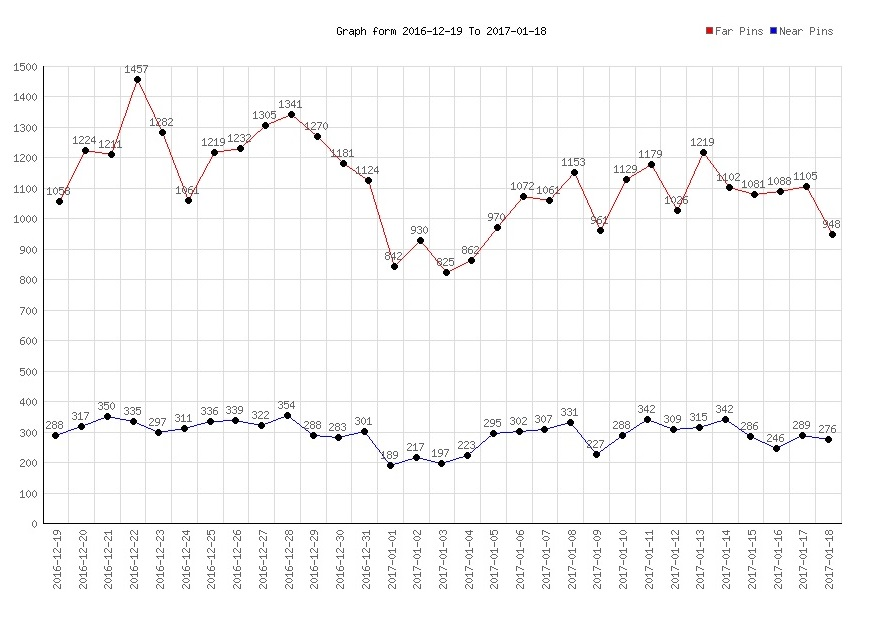
\includegraphics[keepaspectratio, width=125mm]{Graphics/chapter2/pin_graph1.jpg}
       \caption{ピンの周辺と非周辺での乗車実績(1ヶ月)}
       \label{fig:2_2_1}
      \end{minipage}\\
      %---- 2番目の図 --------------------------
      \begin{minipage}[h]{1\hsize}
        \centering
        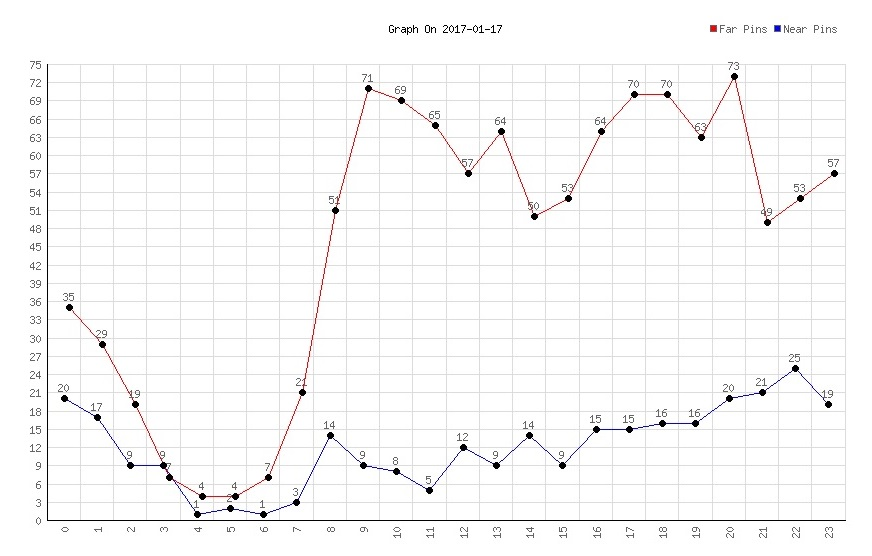
\includegraphics[keepaspectratio, width=125mm]{Graphics/chapter2/pin_graph2.jpg}
       \caption{ピンの周辺と非周辺での乗車実績(1日)}
       \label{fig:2_2_2}
      \end{minipage}
      %---- 図はここまで ----------------------
    \end{tabular}
  \end{figure}

図\ref{fig:2_2_1}と図\ref{fig:2_2_2}はそれぞれ,表示されたピンの周辺と非周辺での乗車実績を1ヶ月スケール(2016年12月19日から2017年1月18日)と1日スケール(2017年1月17日)で示したグラフである.
縦軸が乗客獲得数を表し,横軸が時間を表す.
赤い折れ線は,ピンから離れたところで乗客を獲得した数を表す.
青い折れ線は,ピンの近くで乗客を獲得した数を表す.
乗客を獲得した実績に対するピンの周辺と非周辺の識別は以下のように行った.
営業領域を一辺200mの正方形のセルで分割した.
ピンが1本でも立っているセルがあれば,そのセル自身と,そのセルに隣接するセルはピンの周辺と定義した.
もし,ピンの周辺で乗客を獲得すれば,ピンの近くで乗客を獲得した数を一つ増やした.
そうでなければ,ピンから離れたところで乗客を獲得した数を一つ増やした.

\par
1日スケールのグラフを見ると,朝の3時から6時までの間の乗客獲得数は他の時間帯と比べて少ないことがわかる.
1ヶ月スケールのグラフを見ると,正月三が日の乗客獲得数は他の日に比べて少ないことがわかる.
さらに,どちらのグラフにも共通して言えることがひとつある.
それは,ピンの近くよりもピンから離れたところで乗客を獲得している数が多いということである.
\clearpage

\subsection{ピンに基づいた利己的な走行方向}
\par
図\ref{fig:2_1_1}の画面内にある赤い三角形のオブジェクトは周囲で最もピンがある領域を示す方向を表す.
ピンの情報が表示してあれば,この情報が無くともピンの多い箇所はマップを見ればわかる.
しかし,実際にソフトウェアを利用してみると,マップはある程度拡大表示して利用するため,走行時には周囲のピンの情報を十分に把握することが困難であった.
よって,この利己的な走行方向を示す情報は必要である.
この走行方向は以下の手順で計算した.
まず,営業領域を一辺200mの正方形のセルで分割し,各セルで表示してあるピンの数を数えた.
そして,タクシーがいるセルから3km範囲内でピンの数が3個以上ある一番近いセルを利己的な走行方向とした.
もし,該当するセルが無ければピンの数が2個以下である一番近いセルを利己的な走行方向とした.

\subsection{ピンに基づいた推奨される走行方向}
\par
図\ref{fig:2_1_1}の画面内にある青い三角形のオブジェクトは推奨される走行方向を示すものである.
この走行方向を求めるために,まず,タクシーの移動モデルを混合論理動的システムでモデル化した.
そして,モデル予測制御を応用して最適な移動方向の分布を求め,その分布の中でもっとも大きい値を持つ方向を推奨される走行方向とした.
詳しくは第3章で述べる.

\subsection{ニューラルネットワークを用いた需要予測の結果情報}
\par
ピンの情報は,過去の同曜日,同時刻付近の乗車実績を示していた.
しかし,気象条件を考慮していない.
雨が降ったり,とても暑かったり,寒かったりした場合はタクシーを利用する人が増える傾向がある.
そこで,ニューラルネットワークの入力に天候や気温を含ませて,予測した需要の中で値が大きい箇所を表示することを考えた.
ニューラルネットワークについては付録を参照すること.

\par
ニューラルネットワークは3層とし,以下のような構成にした.
入力層は6つの情報が入力される.
1つ目は月情報のための4個のノードである.
1年を春(3月から5月),夏(6月から8月),秋(9月から11月),冬(12月から2月)の4つに分割して,春であれば春に割り当てられているノードのみに1が与えられ,それ以外のノードには0が与えられる.
2つ目は時刻情報のためのノードである.
24時間は1440分あるので1440個のノードを準備する.
各時刻で対応するノードのみに1が与えられる.
3つ目は祝日であるかどうかのノードである.
祝日であれば1が与えられ,そうでなければ0が与えられる.
4つ目は特別な日であるかどうかのノードである.
大阪のタクシー業界における特別な日とは5日,10日,20日,月末のことである.
タクシー事業者からの聞き取りで,これらの日は仕事でタクシーを利用する人が多く,それ以外の日と乗客数が異なることがわかったため,ノードに追加した.
5つ目は天候に関するノードである.
雨であれば0が与えられ,そうでなければ1が与えられる.
6つ目は気温に関する2つのノードである.
その日の最高気温と最低気温を入力ノードに加えた.
天候と気温の情報は気象庁のサーバーからXML形式またはJSON形式のデータで利用可能だが,事前の登録が必要なため,気象庁のサイトのHTML記述の中からデータ抽出を行った.
入力層のノードの総数は1449個である.
中間層は1層,ノード数は200個とした.
出力層は,タクシーが営業を行う対象領域をいくつかの分割領域に分けたときの,分割領域の個数分だけノードを用意した.
出力層では各分割領域の予測した需要数が出力される.

\par
言語はc++,ライブラリはcaffeを利用し,2016年9月と2016年10月の2ヶ月間の乗車データを使い学習を行った.
セルは一辺200mの正方形とし,ミニバッチ数は100,学習方法は確率的勾配降下法とし,最大学習回数を50000回とした.
ニューラルネットワークに現時刻の2分前から4分後までの時刻や気象情報をそれぞれ入力して,各ノードの出力結果をそれぞれ足し合わせたものを各セルの需要予測数とした.
\begin{figure}[tp]
 \centering
 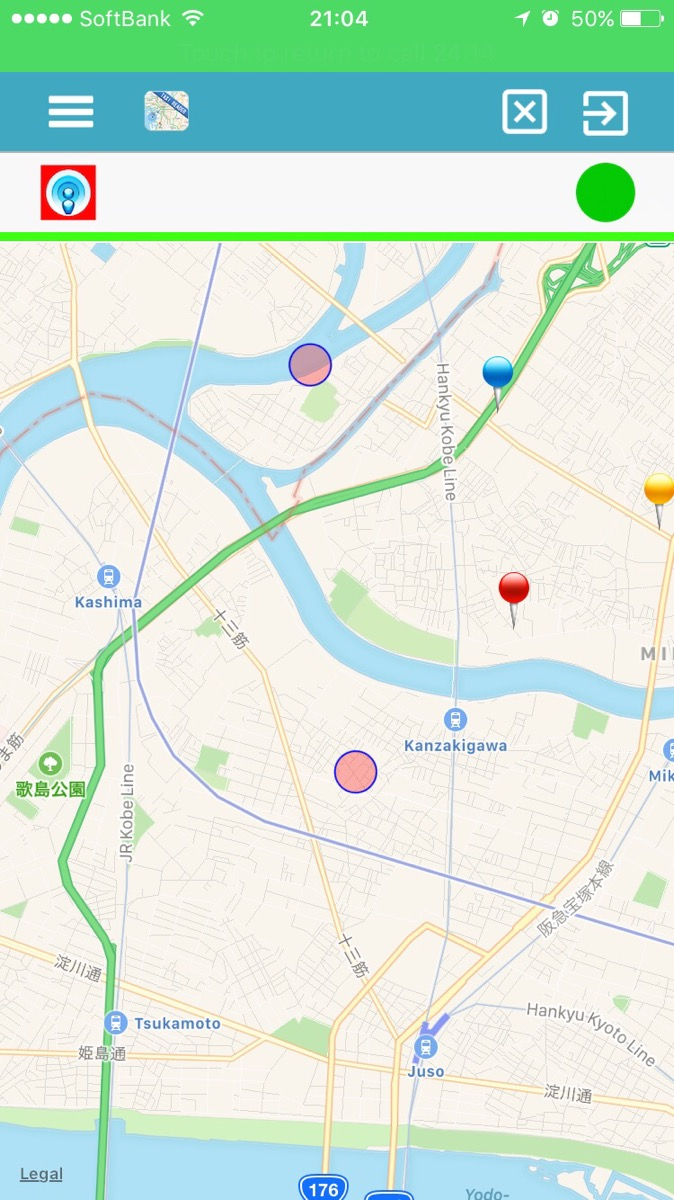
\includegraphics[keepaspectratio, width=60mm]
 {Graphics/chapter2/neural.jpg}
 \caption{ニューラルネットワークで予測した需要が多い箇所の表示方法}
 \label{fig:2_2_4-1}
\end{figure}
需要予測数が1以上あるセルを需要が多い箇所として,
図\ref{fig:2_2_4-1}にあるように,赤いサークルで示した.
本来需要がない川の上に赤いサークルが表示されている.

\clearpage
\subsection{交通情報}
電車の大幅な遅延が発生すると,タクシーやバスなどの他の公共交通機関を利用する人が確実に増える.
そのため,交通情報も乗務員に提示すべき大事な情報である.
インターネット上には,気象情報に限らず交通情報や地震情報のように,時間によって変化するデータが過去のものも含めて公開されている.
今回の実装では,「yahoo!路線情報」のサイトのHTML記述の中からデータ抽出を行い電車の遅延情報を取得し,画面にサイトで表示されている文章を表示することにした.

%  \section{緒言}
%  \par
%  本章では,タクシーの運転支援システムを実現するために企業との共同開発で作成したソフトウェアのシステム構成について説明を行う.
%  ソフトウェアはスマートフォン上で実行され,乗務員に提示される.
%  スマホを利用することでタクシー事業者はカーナビを購入する経費を抑えられるメリットがある.
%  一方,スマホの画面は小さいので,タクシーの乗務員が使いやすいように搭載する機能を選定する必要がある.
%  \section{システム構成}
%  \label{sec:2_2}
% \par

% アプリの主な使い方は以下のとおりである.
% まず,アプリを起動してアプリ上で提供される情報を参考にして流し営業を行い,乗客を乗せた場合は画面右上の緑のサークルをタップする.
% すると,サークルが赤色に変化し,アプリ上でのタクシーのステータスが空車から実車に変化する.
% 乗客を下ろした場合は,もう一度サークルを押してタクシーのステータスを空車に戻す.
% アプリはタクシーのステータスが変化した場合と一定時間・距離走行した場合に位置情報とステータス情報をサーバーに送信する.

% \par
% 提供される情報は以下の5つである.
% 1つ目は営業領域内のイベント情報である.
% 「yahoo!路線情報」のサイトのHTML記述の中からデータ抽出を行い電車の遅延情報を取得し,画面上部に表示する.
% 電車の大幅な遅延が発生すると,タクシーやバスなどの他の公共交通機関を利用する人が確実に増えるため,この情報は重要である.
% 2つ目は過去の同曜日,同時刻付近に乗客を乗せた箇所を示すピン情報である.
% ピンの色は3種類あり,青,黄,赤の順に乗車時間が10分未満,10分以上20分未満,20分以上であった乗降車記録を示している.
% ピンが密集している箇所は乗客を獲得できる頻度が高いと言える.
% 3つ目は周囲で最もピンがある領域を示す方向を表す赤い三角形のオブジェクトである.
% マップを拡大表示して走行していた場合に,周囲のピンを見ることができなくなるので,必要な情報である.
% 4つ目は推奨される走行方向を表す青い三角形のオブジェクトである.
% すべてのタクシーが,ピンが集中している領域に利己的に集まると,それらの領域で供給過多が起きてしまい,全体として乗客獲得の機会を失ってしまう.
% そこで,ピンの情報と空車分布の情報を利用して推奨する走行方向をサーバー側で計算する.
% 5つ目は古典的なニューラルネットワークにより予測した需要の中で需要が多い箇所を表すサークルの情報である.
% 雨が降るとタクシーを利用する人が増える.
% しかし,ピンの表示は気象条件を考慮していない.
% そこで,ニューラルネットワークの入力に天候や気温を含ませて,予測した需要の中で需要が多い箇所を表示することを考えた.

% \par
% 図\ref{fig:fig2_2_2}は4つ目の推奨される走行方向の情報を導き,各乗務員に提示する流れを図化したものである.
% \begin{figure}[hbtp]
%  \centering
%  \includegraphics[keepaspectratio, width=50mm]
%  {Graphics/chapter2/architecture-crop.pdf}
%  \caption{流しタクシーの運転支援システム}
%  \label{fig:fig2_2_2}
% \end{figure}
% 本システムでは,各タクシーから走行データと乗降車データをリアルタイムに受け取り,データベースに保存する.
% 表\ref{tab:tab2_2_3}は実際にデータベースに保存される乗降車データである.
% \begin{table}[hbtp]
%   \begin{center}
%     \caption{データベースに保存される乗降車データ}
%     \begin{tabular}{|l|l|l|l|l|l|} \hline
%       乗車時刻 & 乗車緯度 & 乗車経度 & 降車時刻 & 降車緯度 & 降車経度 \\ \hline \hline
%       2016-11-06 02:18:08 & 34.66128 & 135.50286 & 2016-11-06 02:30:21 & 34.64936 & 135.51944 \\
%       2016-11-06 02:40:40 & 34.66781 & 135.50914 & 2016-11-06 02:47:48 & 34.67094 & 135.53897 \\
%       2016-11-06 03:03:59 & 34.66925 & 135.50633 & 2016-11-06 03:11:49 & 34.67011 & 135.50619 \\ \hline
%     \end{tabular}
%     \label{tab:tab2_2_3}
%   \end{center}
% \end{table}
% 需要予測器では,表\ref{tab:tab2_2_3}の履歴データから乗客の発生分布を予測する.
% 最適化器では,モデル予測制御を用いて,この乗客予測と現在の空車のタクシーの分布から最適なタクシーの移動分布を求める.

% \par
% 5つ目の情報を計算するためのニューラルネットワークは以下のような構成にした.
% 入力層は6つの情報が入力される.
% 1つ目は月情報のための4個のノードである.
% 1年を春(3月から5月),夏(6月から8月),秋(9月から11月),冬(12月から2月)の4つに分割して,春であれば春に割り当てられているノードのみに1が与えられ,それ以外のノードには0が与えられる.
% 2つ目は時刻情報のためのノードである.
% 24時間は1440分あるので1440個のノードを準備する.
% 各時刻で対応するノードのみに1が与えられる.
% 3つ目は祝日であるかどうかのノードである.
% 祝日であれば1が与えられ,そうでなければ0が与えられる.
% 4つ目は特別な日であるかどうかのノードである.
% 大阪のタクシー業界における特別な日とは5日,10日,20日,月末のことである.
% タクシー事業者からの聞き取りで,これらの日は仕事でタクシーを利用する人が多く,それ以外の日と乗客数が異なることがわかったため,ノードに追加した.
% 5つ目は天候に関するノードである.
% 雨であれば0が与えられ,そうでなければ1が与えられる.
% 6つ目は気温に関する2つのノードである.
% その日の最高気温と最低気温を入力ノードに加えた.
% 天候と気温の情報は気象庁のサーバーからXML形式またはJSON形式のデータで利用可能だが,イベント情報の時と同様に,サイトのHTML記述の中からデータ抽出を行った.
% 入力層のノードの総数は1449個である.
% 中間層は1層,ノード数は200個とした.
% 出力層は,タクシーが営業を行う対象領域をいくつかの分割領域に分けた時に,それぞれの分割領域の需要数を予測するために分割領域の数のノードを用意した.

%  \section{結言}
%  \label{sec:2_3}
%  \par
%  本章では,提案するアプリケーションのシステム構成について説明を行った.
%  乗務員には周辺のイベント情報と,過去に乗客を乗せた箇所を示すピン情報と,周辺で最もピンがある領域を示す方向と,推奨される進行方向と,古典的なニューラルネットワークにより予測した需要の中で需要が多い箇所を表すサークルの情報を示す.
%  イベント情報や需要予測に用いる気象情報などはインターネット上から取得する.
%  インターネット上には気象情報のように時間によって変化するデータが過去のものも含めて公開されている.
%  データの形式はXML形式やJSON形式のようにプログラムからの利用を考慮したものや,HTML記述のものもある.
%  気象庁や国土交通省のような公的な機関が提供するデータだけではなく,SNSなどの手段を利用して得られたリアルタイムな情報をイベント情報として提供することも考えられる.
%  また,需要予測器として古典的なニューラルネットワークを利用したが,学習データにスパーク性があるため過学習を起こす問題がある.
% 多変量時系列モデルのような他の予測方法もあるため,タクシー運転支援システムの実装に適した需要予測の方法を見つけることが,今後の研究課題である.

 \end{document}